\documentclass[
%% TIKZ_CLASSOPTION %%
tikz
]{standalone}
\usepackage{amsmath}
\usetikzlibrary{matrix}
%% EXTRA_TIKZ_PREAMBLE_CODE %%
\begin{document}
%% TIKZ_CODE %%
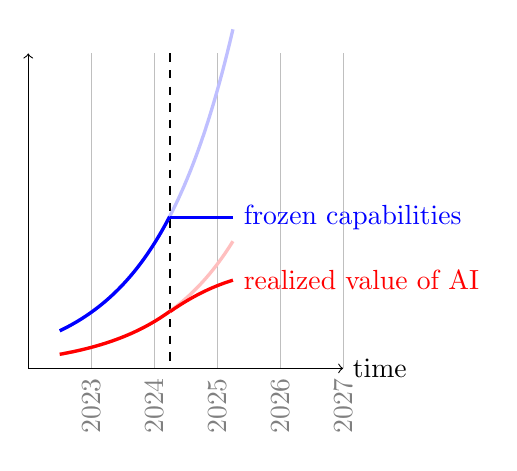
\begin{tikzpicture}[scale=4]
  \draw[<->] (1,0)  node[right] {time}--(0,0) -- (0,1);
  \draw[gray!50!white] (.2,1)--(.2,0) node[left,rotate=90,gray] {2023};
  \draw[gray!50!white] (.4,1)--(.4,0) node[left,rotate=90,gray] {2024};
  \draw[gray!50!white] (.6,1)--(.6,0) node[left,rotate=90,gray] {2025};
  \draw[gray!50!white] (.8,1)--(.8,0) node[left,rotate=90,gray] {2026};
  \draw[gray!50!white] (1,1)--(1,0) node[left,rotate=90,gray] {2027};
  \draw[dashed] (0.45,1)--(0.45,0);
  \draw[domain=0.1:.65,smooth,samples=100,blue!25!white,very thick] plot (\x,{0.08*exp(4*\x)});
  \draw[domain=0.1:.45,smooth,samples=100,blue,very thick] plot (\x,{0.08*exp(4*\x)});
  \draw[blue,very thick] (0.45,0.48)--(0.65,0.48)  node[right,align=left] {frozen capabilities};

  \draw[domain=0.1:.65,smooth,samples=100,red!25!white,very thick] plot (\x,{0.03*exp(4*\x)});
  \draw[domain=0.1:.45,smooth,samples=100,red,very thick] plot (\x,{0.03*exp(4*\x)});
  \draw[red,very thick] plot[smooth,tension=1] coordinates{(0.45,0.18) (0.55,0.24) (0.65,0.28)}
      node[right,align=left] {realized value of AI};
\end{tikzpicture}
\end{document}
